\newpage
\section{A3.1}

Consider the directed graph $G = \langle V,\ E\rangle$ given by vertices $V =
\{A,\ B,\ C,\ D\}$ and edges:

\begin{alignat*}{5}
  E = \{&(A,\ B),\ (A,\ C),\ (B,\ C),\ (B,\ D),\\[4pt]
        &(C,\ A),\ (C,\ D),\ (D,\ D)\}\\[4pt]
\end{alignat*}

where $(X,\ Y)$ denotes a directed edge with source $X$ and sink $Y$.

\subsection{A3.1.a}

\begin{itemize}
  \item \emph{Reproduce the graph $G$ using Graphviz.}
\end{itemize}

I write the following Graphviz code to reproduce the graph:

\begin{minted}[linenos=false]{text}
digraph task1 {
  A -> B, C
  B -> C, D
  C -> A, D
  D -> D
}
\end{minted}

Compiling this to a graph using \ms{dot}, I get the below graph:

\begin{figure}[H]
  \centering

  \includegraphics[width=2cm]{../task1.png}
\end{figure}

\sectend


\newpage
\subsection{A3.1.b}

\begin{itemize}
  \item \emph{Reproduce the graph $G$ in \LaTeX ~using a graphics package.}
\end{itemize}

I choose Tikz, since that it the only latex package for graph drawing that I
have any experience with. I write the below latex code:

\begin{minted}[highlightlines={2-4, 8-10, 18}]{tex}
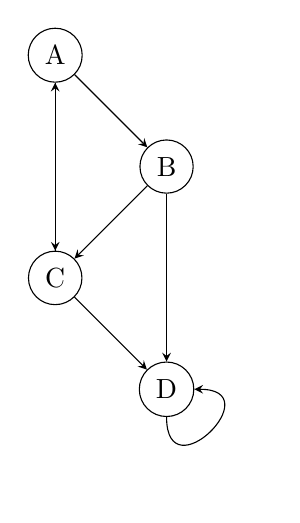
\begin{tikzpicture}
  [v/.style={draw, circle}, % draw circles around nodes.
  node distance = 2cm,      % add some spacing between nodes.
  > = stealth               % prettier arrows.
  ]

  \node[v] (A) {A};
  \node[v] (B) [below right of = A] {B};
  \node[v] (C) [below left  of = B] {C};
  \node[v] (D) [below right of = C] {D};

  \draw[->] (A) to (B);
  \draw[->] (A) to (C);
  \draw[->] (B) to (C);
  \draw[->] (B) to (D);
  \draw[->] (C) to (A);
  \draw[->] (C) to (D);
  \draw[->] (D) to [out=270, in=0, looseness=5] (D);
\end{tikzpicture}
\end{minted}

Which produces this graph:

\smallskip

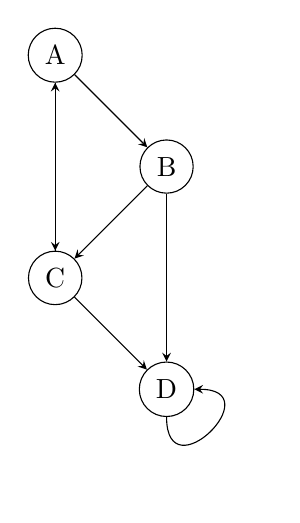
\begin{tikzpicture}
  [v/.style={draw, circle}, % draw circles around nodes.
  > = stealth,              % prettier arrows.
  node distance = 2cm       % add some spacing between nodes.
  ]

  \node[v] (A) {A};
  \node[v] (B) [below right of = A] {B};
  \node[v] (C) [below left  of = B] {C};
  \node[v] (D) [below right of = C] {D};

  \draw[->] (A) -- (B);
  \draw[->] (A) -- (C);
  \draw[->] (B) -- (C);
  \draw[->] (B) -- (D);
  \draw[->] (C) -- (A);
  \draw[->] (C) -- (D);
  \draw[->] (D) to [out=270, in=0, looseness=5] (D);
\end{tikzpicture}

\emph{Notice that the edge between nodes $A$ and $C$ is bi-directional.}


\newpage
\subsection{A3.1.c}

\begin{itemize}
  \item \emph{Discuss the effort of making the graph drawings using Graphviz as
    compared to using Tikz.}
\end{itemize}

First off, drawing the graph in Graphviz obviously took a lot less effort and
lines of code than using Tikz - this is clearly evidenced by the amount of code
taken to generate the two (6 lines and 17 lines for Graphviz and Tikz,
respectively).

\medskip

The sheer number of lines of code is, of course, not a big problem in and of
itself - verbose code does not always have to be complex code. However, I
identify a handful of problems with working with Tikz that are \emph{not}
problems in Graphviz.

% \begin{itemize}
%   \item \emph{having to declare vertices and edges separately.}
% \end{itemize}


\paragraph{Declaring vertices and edges}~\smallskip

In Tikz, vertices and edges in the graph must be declared separately, and any
number of edges leaving a single vertex must similarly be declared separately.

\medskip

In Graphviz, two vertices \ms{A} and \ms{B} with a directed edge from \ms{A} to
\ms{B} is declared simply with the syntax \ms{A -> B}. If either of the vertices
do not already exist, then it does after the declaration. Additionally, if one
vertex is to have multiple outgoing edges, then these can be declared
simultaneously with the notation \ms{A -> B, C}.

\smallskip

It is also possible to declare vertices separately from declaring their edges.
This is for example necessary if multiple vertices are to have the same name
(since otherwise the name is also used for internal identification).

\paragraph{Positioning of elements in the graph}~\smallskip

In Tikz, the user is not \emph{forced} to specify positioning, but any vertices
for which position is not specified will be placed on top of one another,
whereas in Graphviz, vertices are positioned automatically with at least some
reasonable amount of spacing if the user does not manually specify positioning.

\paragraph{Special edges}~\smallskip

The graph $G$ contains an edge from $D$ to $D$. In Graphviz, this is encoded
with simply \ms{D -> D}. To properly encode this edge in Tikz, we have to
specify start and end points for the edge, and we must give these in radians on
the circumference of the in/out vertices. 

\smallskip

As an example, the below latex code:

\begin{minted}{tex}
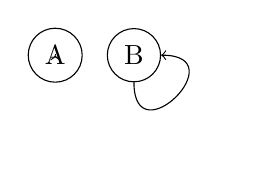
\begin{tikzpicture}
  [v/.style={draw, circle}]

  \node[v] (A) {A};
  \node[v] (B) [right of = A] {B};

  \draw[->] (A) to (A);
  \draw[->] (B) to [out=270, in=0, looseness=5] (B);
\end{tikzpicture}
\end{minted}

generates this graph:

\smallskip

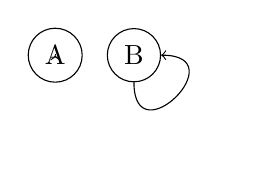
\begin{tikzpicture}
  [v/.style={draw, circle}]

  \node[v] (A) {A};
  \node[v] (B) [right of = A] {B};

  \draw[->] (A) to (A);
  \draw[->] (B) to [out=270, in=0, looseness=5] (B);
\end{tikzpicture}

\emph{Notice how the in- and outgoing arrows on vertex $A$ are placed on top of
another on the top of the vertex.}


\sectend

\subsection{A3.1.d}

\begin{itemize}
  \item \emph{With Graphviz, adding a single edge to a graph can in some cases
    significantly alter the layout of that graph. Discuss advantages and
    disadvantages of this.}
\end{itemize}

When drawing graphs, Graphviz will always attempt to draw the graph such that
there are no edges intersecting. This is, of course, only possible when the
graph is planar, but often even a planar graph must be carefully rearranged to
be drawn on a 2D surface with no intersections.

\smallskip

Even if adding an edge to a planar graph results in a planar graph, it is often
necessary to rearrange the graph to avoid intersections, and potentially even to
the point of the graph becoming unrecognizable. As such, I would argue that it
is very permissible for Graphviz to sometimes drastically alter a graph when an
edge is added.

\medskip

Additionally, it is often very convenient to not have to position vertices
manually when drawing a graph. This becomes increasingly helpful when adding
graphs to already existing, large graphs.

\medskip

However, drawing a graph with intersections can sometimes be preferable to
rearranging it even if the graph is planar - for example if some features of the
graph are only visually obvious when the graph is arranged in a certain way. In
such cases it can be an enormous annoyance to not control over vertex placement
- fortunately, however, Graphviz (like Tikz and basically every other graph
drawing utility out there) supports manual positioning of vertices.

\Sectend
